\documentclass[12pt]{scrartcl}

 

\usepackage{float}

\usepackage[utf8]{inputenc}

\usepackage[T1]{fontenc}

\usepackage{lmodern}

\usepackage[ngerman]{babel}

\usepackage{amsmath}

\usepackage{graphicx}


 

\title{Versuch MI1\\ Mikrowellen}

\author{Frederik Strothmann, Henrik Jürgens}

\date{\today}


\begin{document}


 %deckblatt erstellen

\maketitle
\tableofcontents
\newpage

%einleitung zu dem experiment

\section{Einleitung}

Ein System aus Mikrowellensender und verschiedenen Empfängern ermöglicht Untersuchungen verschiedener physikalischer Effekte an Mikrowellen. So sollen in diesem Versuch stehende Wellen vermessen werden, außerdem wird die Wirkung einer Wachs-Sammellinse oder eines Polfilters (parallele Metallstäbe) untersucht sowie die Reflexion
an einer Wachsplatte (Brewster-Winkel), die Totalreflexion zwischen einer Wachs-Luft-
Wachs-Schicht und die Drehung der Polarisationsebene durch
”optisch aktive“ Substanzen.
(Spiralfedern in einem Styroporträger)
%versuchsaufbau mit skizze

\section{Versuchsaufbau}
Der Versuchsaufbau besteht aus einem Mikrowellen Sender und Empfänger, einer Wachslinse, einem Wachsquader, zwei Wachsprismen, einem Gitter und einem Netzgerät. Zum messen der Intensität waren ein DMM und ein Amperemeter mit integriertem Strahlenempfänger vorhanden.Sender und Empfänger sind in zwei Halterungen angebracht, welche mit einer Winkelskala versehen sind.
Der Versuchsaufbau besteht aus einem Mikrowellen Sender und Empfänger, einer Wachslinse, einem Wachsquader, zwei Wachsprismen, eine Gmitter und einem Netzgerät. Zum messen der Intensität waren ein DMM und ein Amperemeter mit integriertem Strahlenempfänger vorhanden. Sender und Empfänger waren in zwei Halterungen angebracht, welche mit einer Winkelskala versehen sind.


\begin{figure}[H]
	\centering
	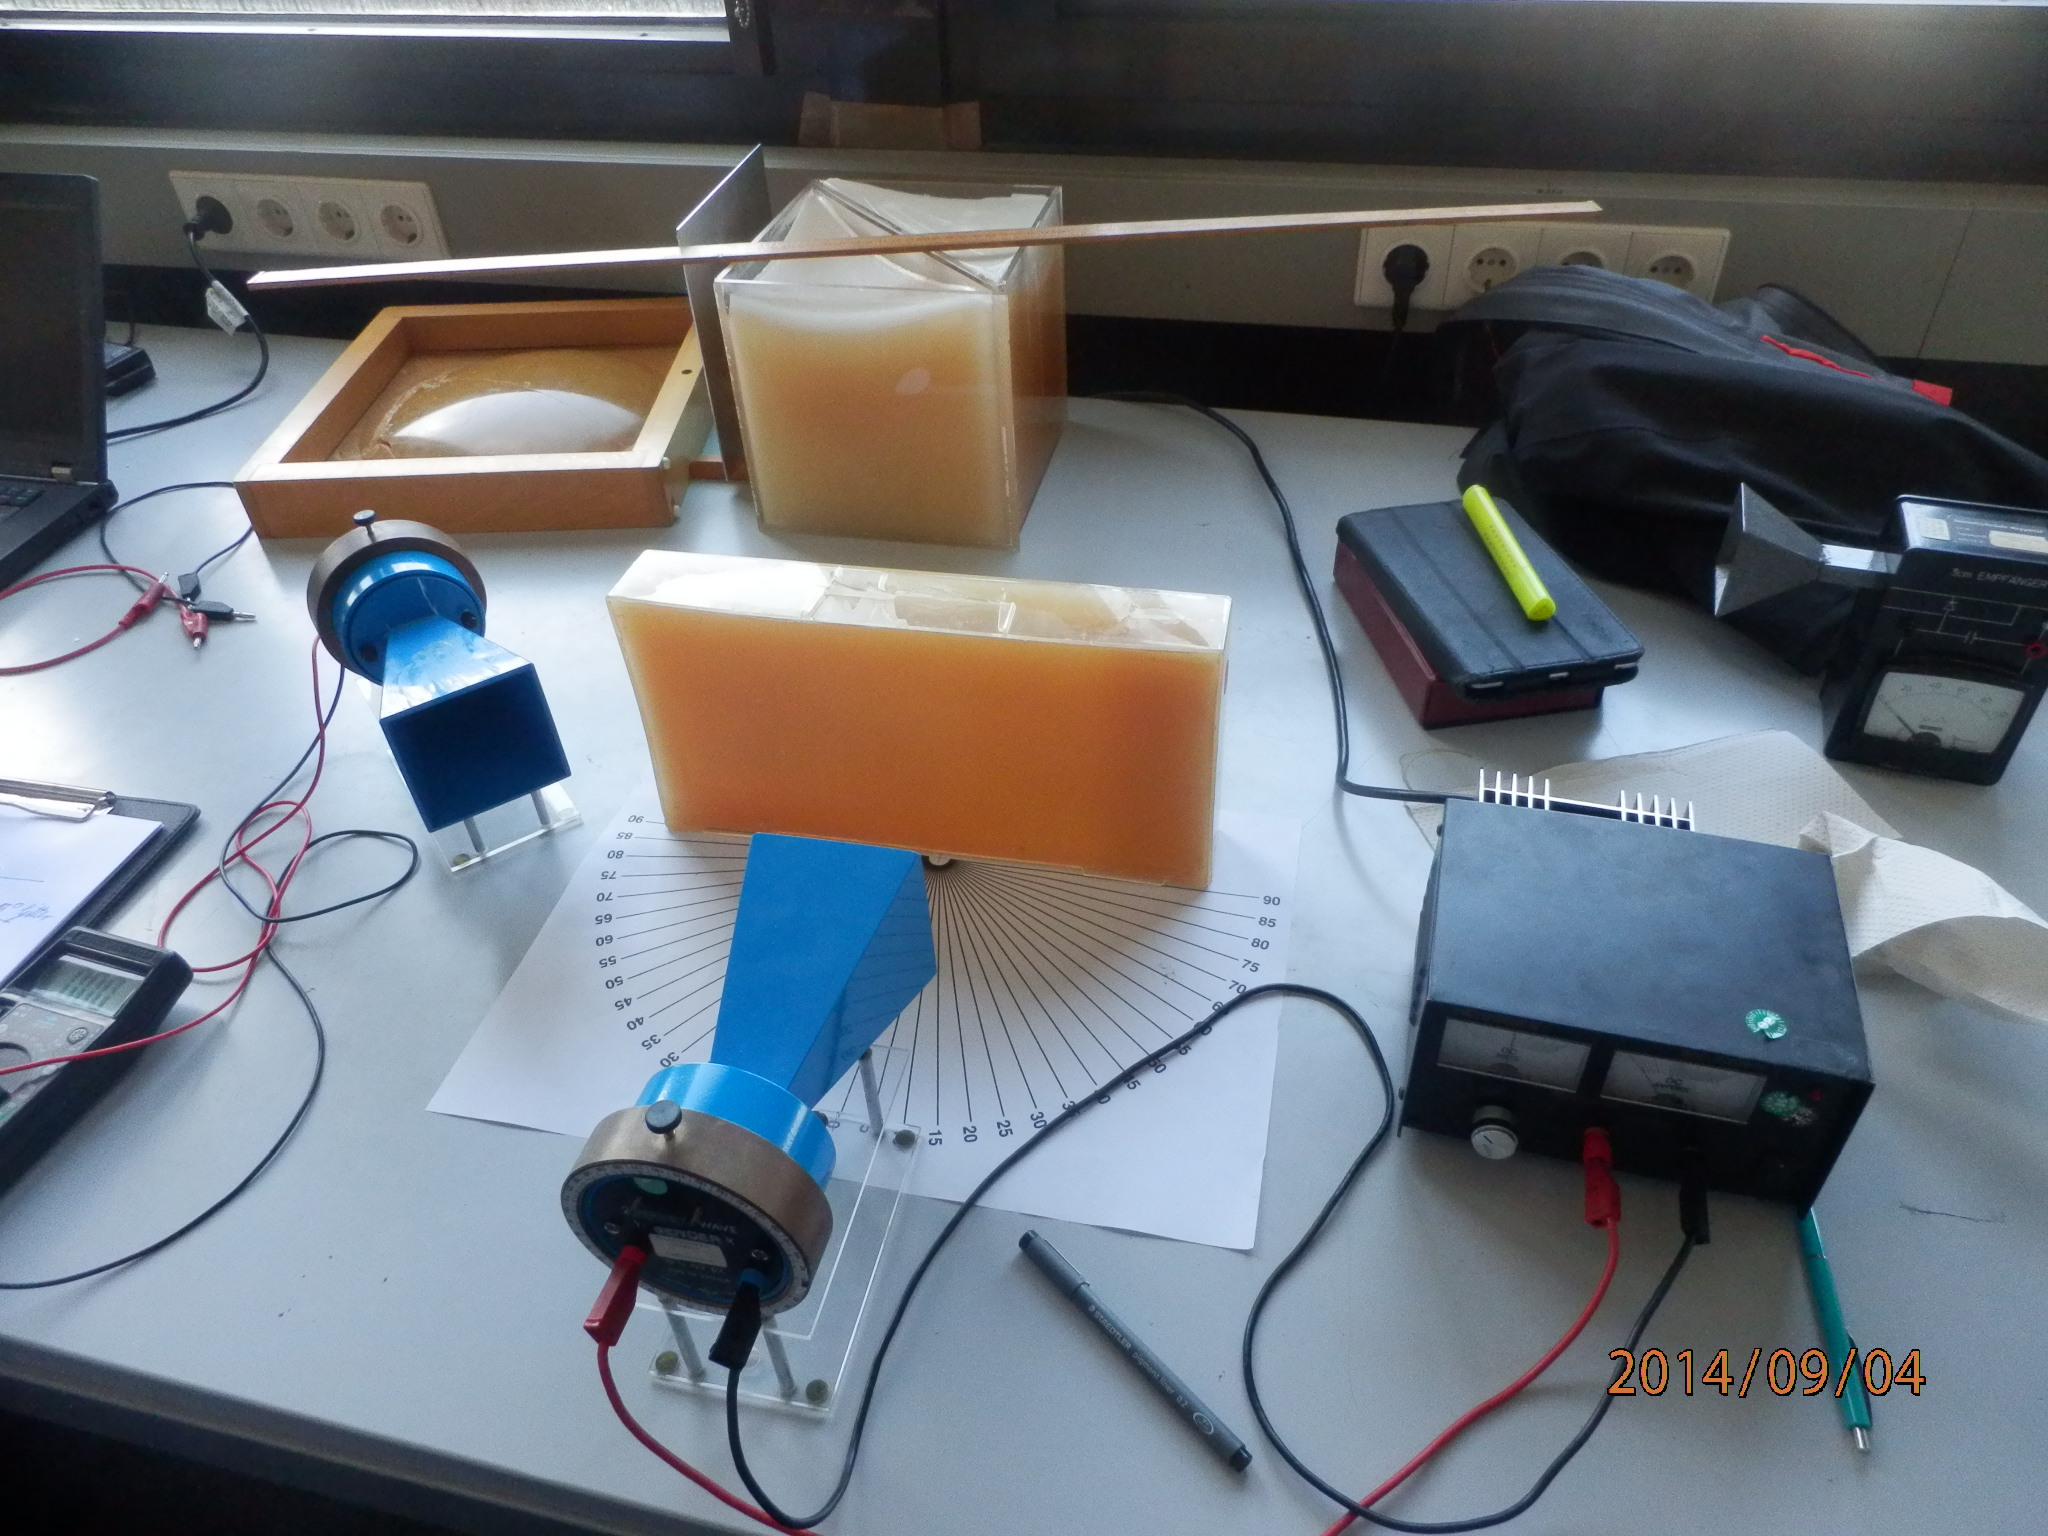
\includegraphics[scale= 0.1]{versuchaufbau.JPG}
	\label{fig:versuchsaufbau}
\end{figure}

%wenn du tabellen einfügst dann schreib bitte anstatt [htpb] [H]. zusammen mit \usepackage{float} verrutscht dann garnichts mehr
Die Mikrowellensender werden mit einer Gleichspannung von ca. 10 bis 12 V versorgt.
\section{Aufgabe1}
\subsection{Versuchsdurchführung}
\subsubsection{Praktische Durchführung}
Zunächst stellen wir den Sender und eine Metallplatte im Abstand von ca. 30 - 40 cm gegenüber auf und zwischen beide die Diode. Dadurch bildet sich eine stehende Welle, sodass wir durch Verschieben der Metallplatte die Wellenlänge messen können.
\subsubsection{Theoretische Durchführung}
Die Wellenlänge wird bestimmt nach Formel:
\begin{align}
n\lambda = p_1 - p_2
\label{eqn:a_1}
\end{align}
n ist dabei die Anzahl der Minima zwischen den Positionen $p_1$ und $p_2$.\\
Mit einem Fehler von:
\begin{align}
\sigma_{\lambda} = \sqrt{
\left(\frac{\sigma_{p_1}}{n}\right)^2+
\left(\frac{\sigma_{p_2}}{n}\right)^2}
\label{eqn:a_1_sigma}
\end{align}
\subsection{Messergebnisse}
\begin{table}[H]
\caption{Abstandsmessungen der ersten Aufgabe, der Fehler beträgt bei allen Werten $(\pm 0,005)$}
\centering
\begin{tabular}{|r|}
\hline
\multicolumn{1}{|l|}{d/m} \\ \hline
0,36 \\ \hline
0,3735 \\ \hline
0,387 \\ \hline
\end{tabular}
\label{tab:a_1}
\end{table}
\subsection{Auswertung}
In der ersten Aufgabe sollte die Wellenlänge des Senders bestimmt werden. Dabei wurden drei verschiedene Positionen gemessen (siehe Tabelle \ref{tab:a_1}). Die Wellenlänge wurde mit Gleichung \ref{eqn:a_1} und der Fehler mit Gleichung \ref{eqn:a_1_sigma} bestimmt. Es ergab sich ein Mittelwert von:
\begin{align*}
2,7 (\pm 0,2) cm
\end{align*}
Auf dem Sender war ein Wert von 2,8 cm für die Wellenlänge angegeben.
\subsection{Diskussion}
Die auf dem Sender angegebene Wellenlänge liegt im ersten Sigmaintervall der gemessenen Wellenlänge, wobei der Fehler weniger als 8\% des Messwertes einnimmt. Auf diese Weise konnte die Wellenlänge also relativ genau bestimmt werden.
\section{Aufgabe2}
\subsection{Versuchsdurchführung}
\begin{figure}[H] 
  \centering
    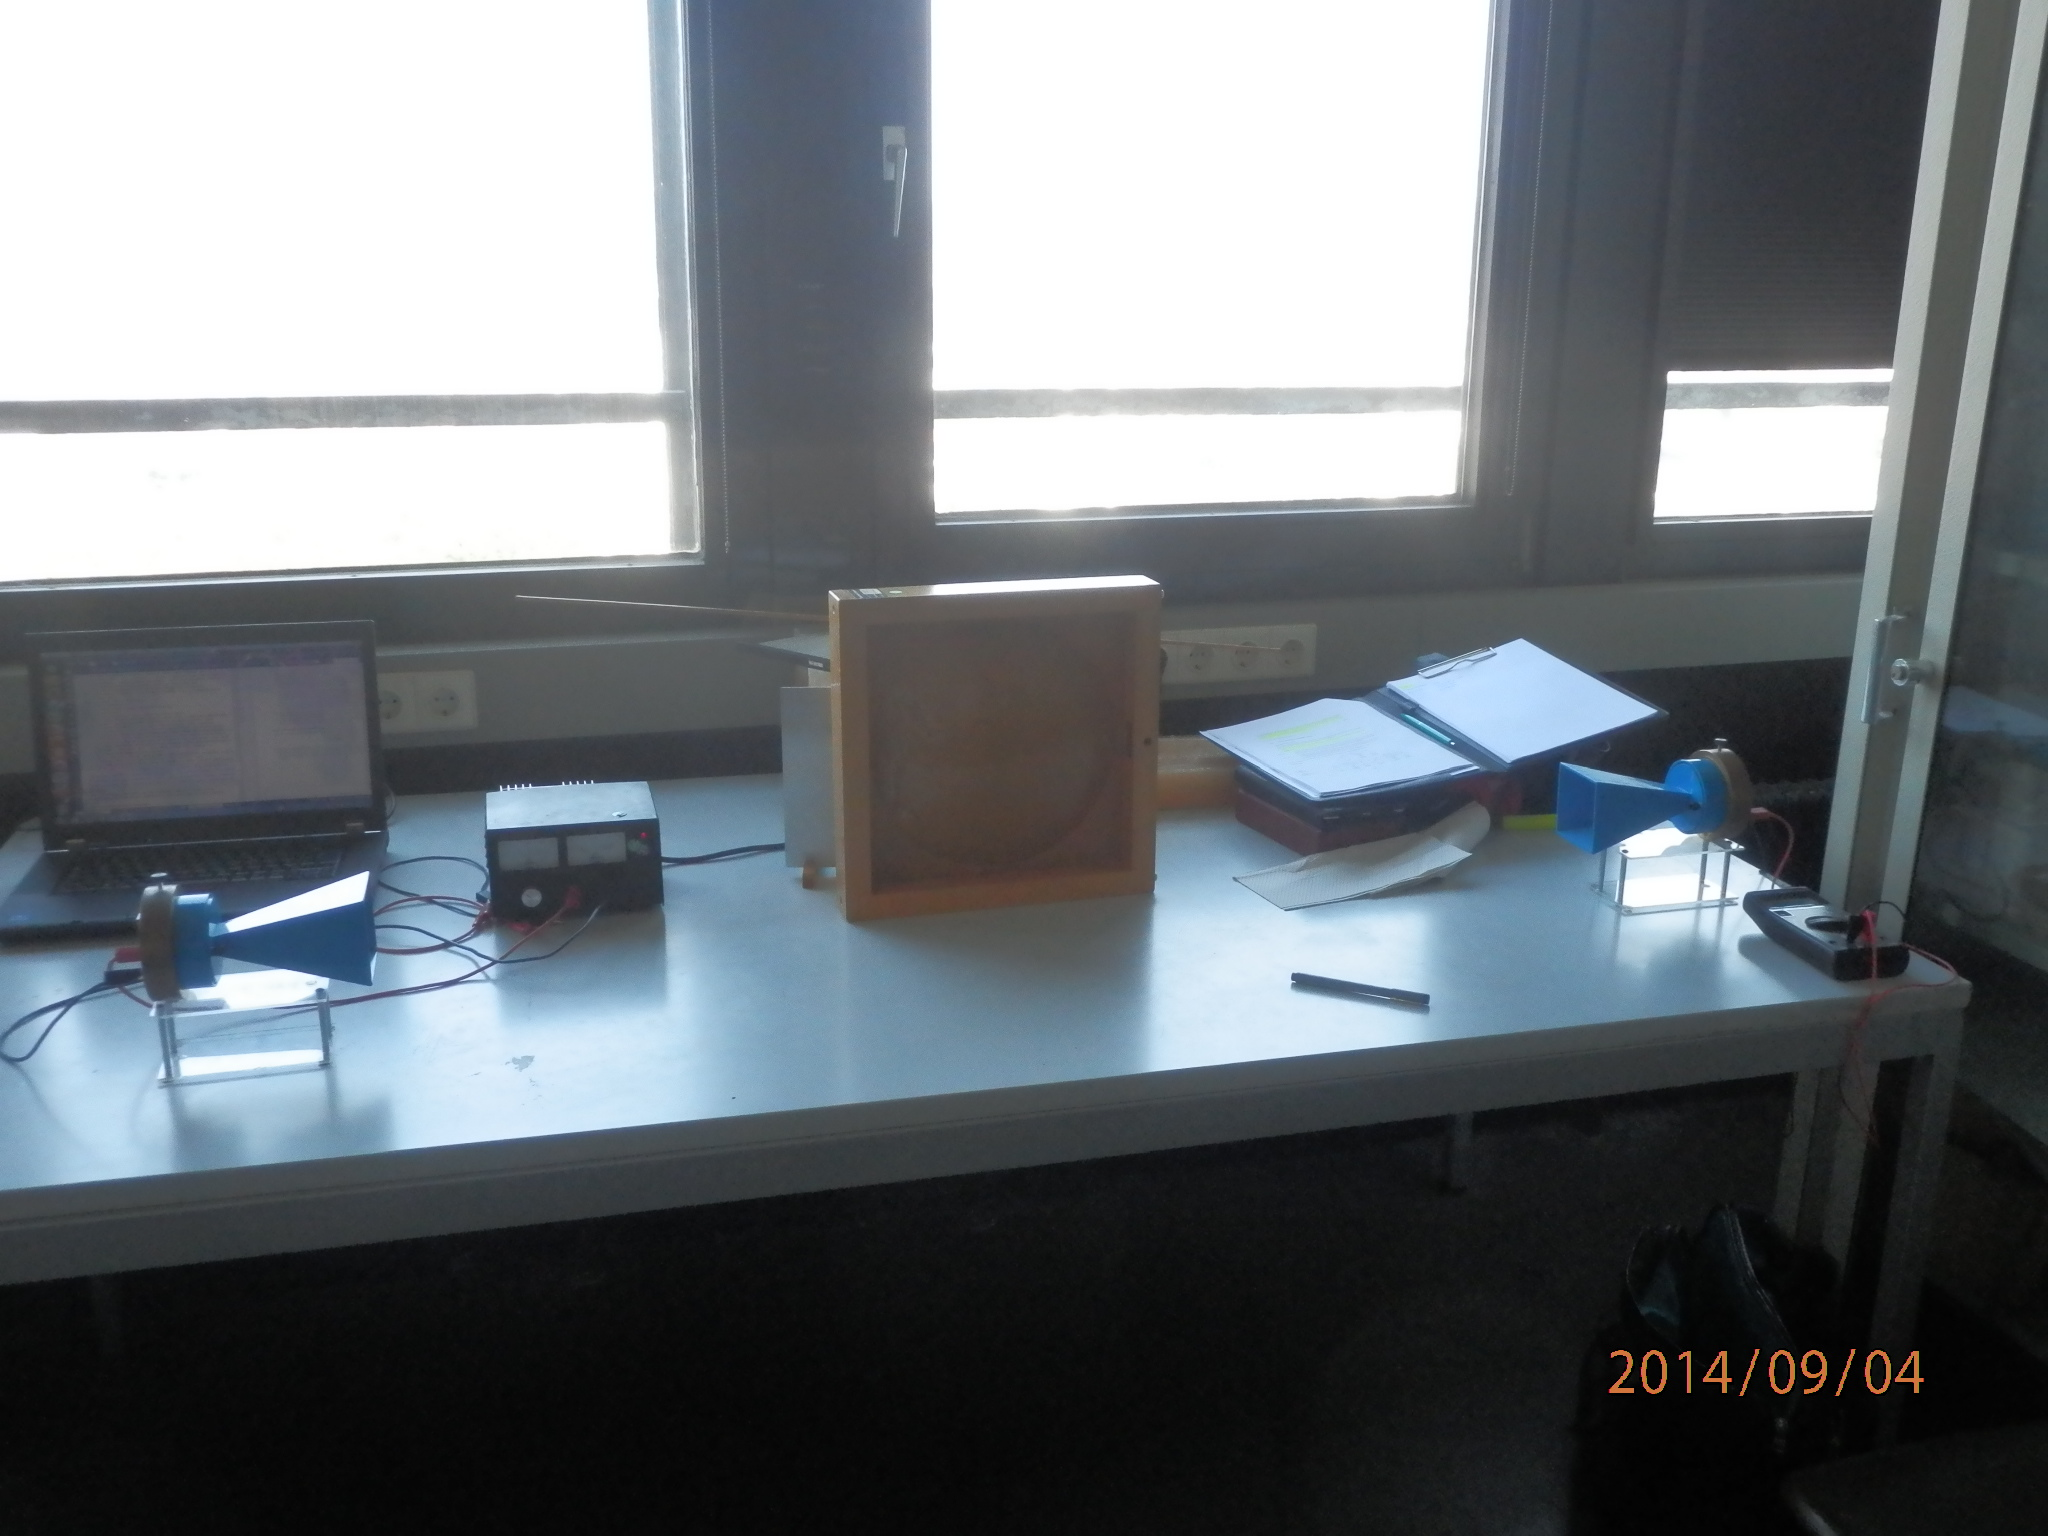
\includegraphics[scale = 0.1]{a_2.JPG}
  	\caption[Aufbau des zweiten Versuchs]{Aufbau des zweiten Versuchs}
  \label{fig:a_2}
\end{figure}
\subsubsection{Praktische Durchführung}
Wir messen die Intensitätsverteilung senkrecht zur Strahlrichtung mit dem Hornempfänger, wobei uns eine Wachslinse zur Verfügung stand:
\begin{enumerate}
\item ohne Linse (Abstand Sender-Empfänger ca. 1,5 m)
\item mit Linse (Abstand Sender-Linse 0,5 m, Linse-Empfänger 1 m)
\end{enumerate}
\subsection{Messergebnisse}
\begin{table}[H]
\caption{Daten der Messung ohne Linse. Für den Fehler des Stromes wurde ein Wert von $(\pm 1)$ A und für die Positon wurde ein Fehler von $(\pm 0,1)$ cm angenommen.}
\centering
\begin{tabular}{|r|r|}
\hline
\multicolumn{1}{|l|}{Strom/$\mu$A} & \multicolumn{1}{l|}{p/cm} \\ \hline
67 & 0 \\ \hline
68 & -1 \\ \hline
65 & -2 \\ \hline
63 & -3 \\ \hline
61 & -4 \\ \hline
61 & -5 \\ \hline
71 & 1 \\ \hline
70 & 2 \\ \hline
69 & 3 \\ \hline
68 & 4 \\ \hline
68 & 5 \\ \hline
\end{tabular}
\label{tab:a_2_o}
\end{table}

\begin{table}[H]
\caption{Daten der Messung mit Linse. Für den Fehler des Stromes wurde ein Wert von $(\pm 1)$ A und für die Positon wurde ein Fehler von $(\pm 0,1)$ cm angenommen.}
\centering
\begin{tabular}{|r|r|}
\hline
\multicolumn{1}{|l|}{Strom/$\mu$A} & \multicolumn{1}{l|}{p/cm} \\ \hline
53 & 0 \\ \hline
52 & -1 \\ \hline
51 & -2 \\ \hline
50 & -3 \\ \hline
47 & -4 \\ \hline
44 & -5 \\ \hline
50 & 1 \\ \hline
48 & 2 \\ \hline
45 & 3 \\ \hline
42 & 4 \\ \hline
40 & 5 \\ \hline
\end{tabular}
\label{tab:a_2_m}
\end{table}
\subsection{Auswertung}
In der zweiten Aufgabe sollte der Effekt einer Sammellinse überprüft werden.
Dafür wurden Sender und Empfänger in einem Abstand von 1,5 Metern zueinander aufgestellt und die Intensität entlang der Orthogonalen vermessen. Dies geschah einmal mit der Sammellinse dazwischen und einmal ohne. Für die Messung ohne Sammellinse ergab sich der folgende Plot (Messwerte aus Tabelle \ref{tab:a_2_o}). p ist  bei beiden Versuchsteilen der Abstand des Empfängers zu Intensitätsmaximum.

\begin{figure}[H]
\centering
    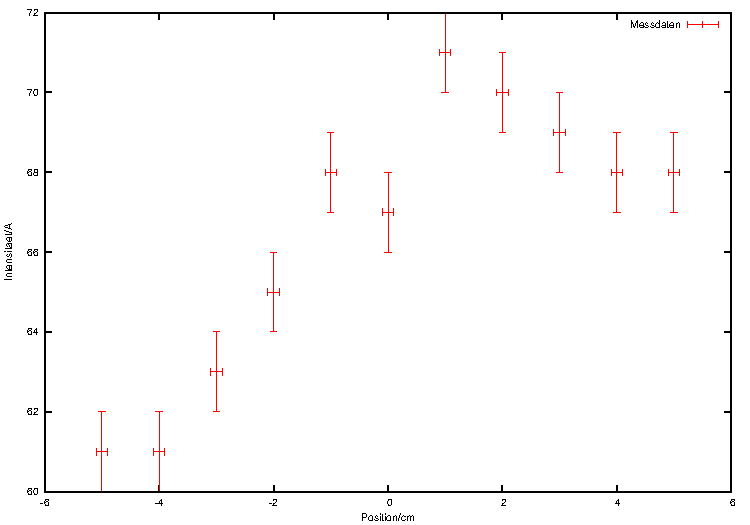
\includegraphics[scale = 1]{a_2_o.pdf}
  	\caption[Plot der Messung ohne Sammellinse]{Plot der Messung ohne Sammellinse}
  \label{fig:a_2_o}
\end{figure}

Bei der Messung mit Sammellinse ergab sich der folgende Plot (Messwerte aus Tabelle \ref{tab:a_2_m}).


\begin{figure}[H]
\centering
    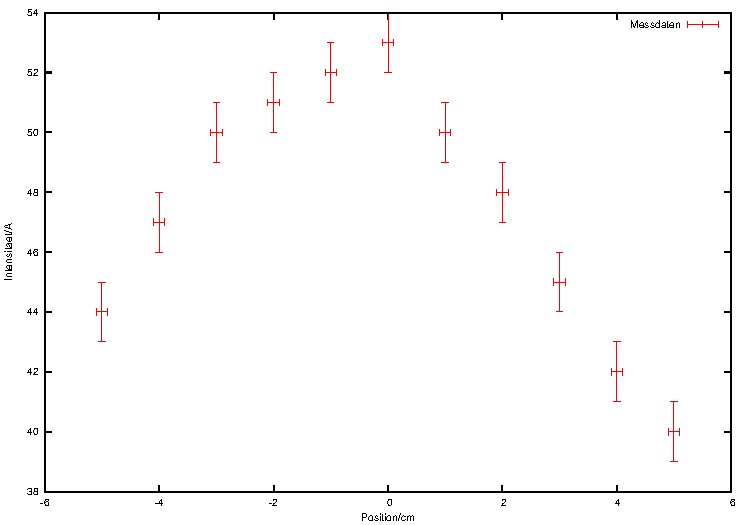
\includegraphics[scale = 1]{a_2_m.pdf}
  	\caption[Plot der Messung mit Sammellinse]{Plot der Messung mit Sammellinse}
  \label{fig:a_2_m}
\end{figure}
\subsection{Diskussion}
Obwohl unsere Linse einige Bruchstellen hatte und unser DMM mehr oder weniger defekt war, da es bei umschalten der Zehnerpotenzen ganz andere Ströme anzeigte,(wir haben die Einstellung benutzt, bei der die Ergebnisse vergleichbar mit denen der Nachbargruppe waren,) kann man an dem Plot erkennen, dass der Lichtstrahl durch die Linse fokussiert wurde und die Steigung, also die Abnahme der Intensität mit zunehmendem Abstand zum Mittelpunkt mit Linse größer war als ohne.
\section{Aufgabe3}
\subsection{Versuchsdurchführung}
\begin{figure}[H] 
  \centering
    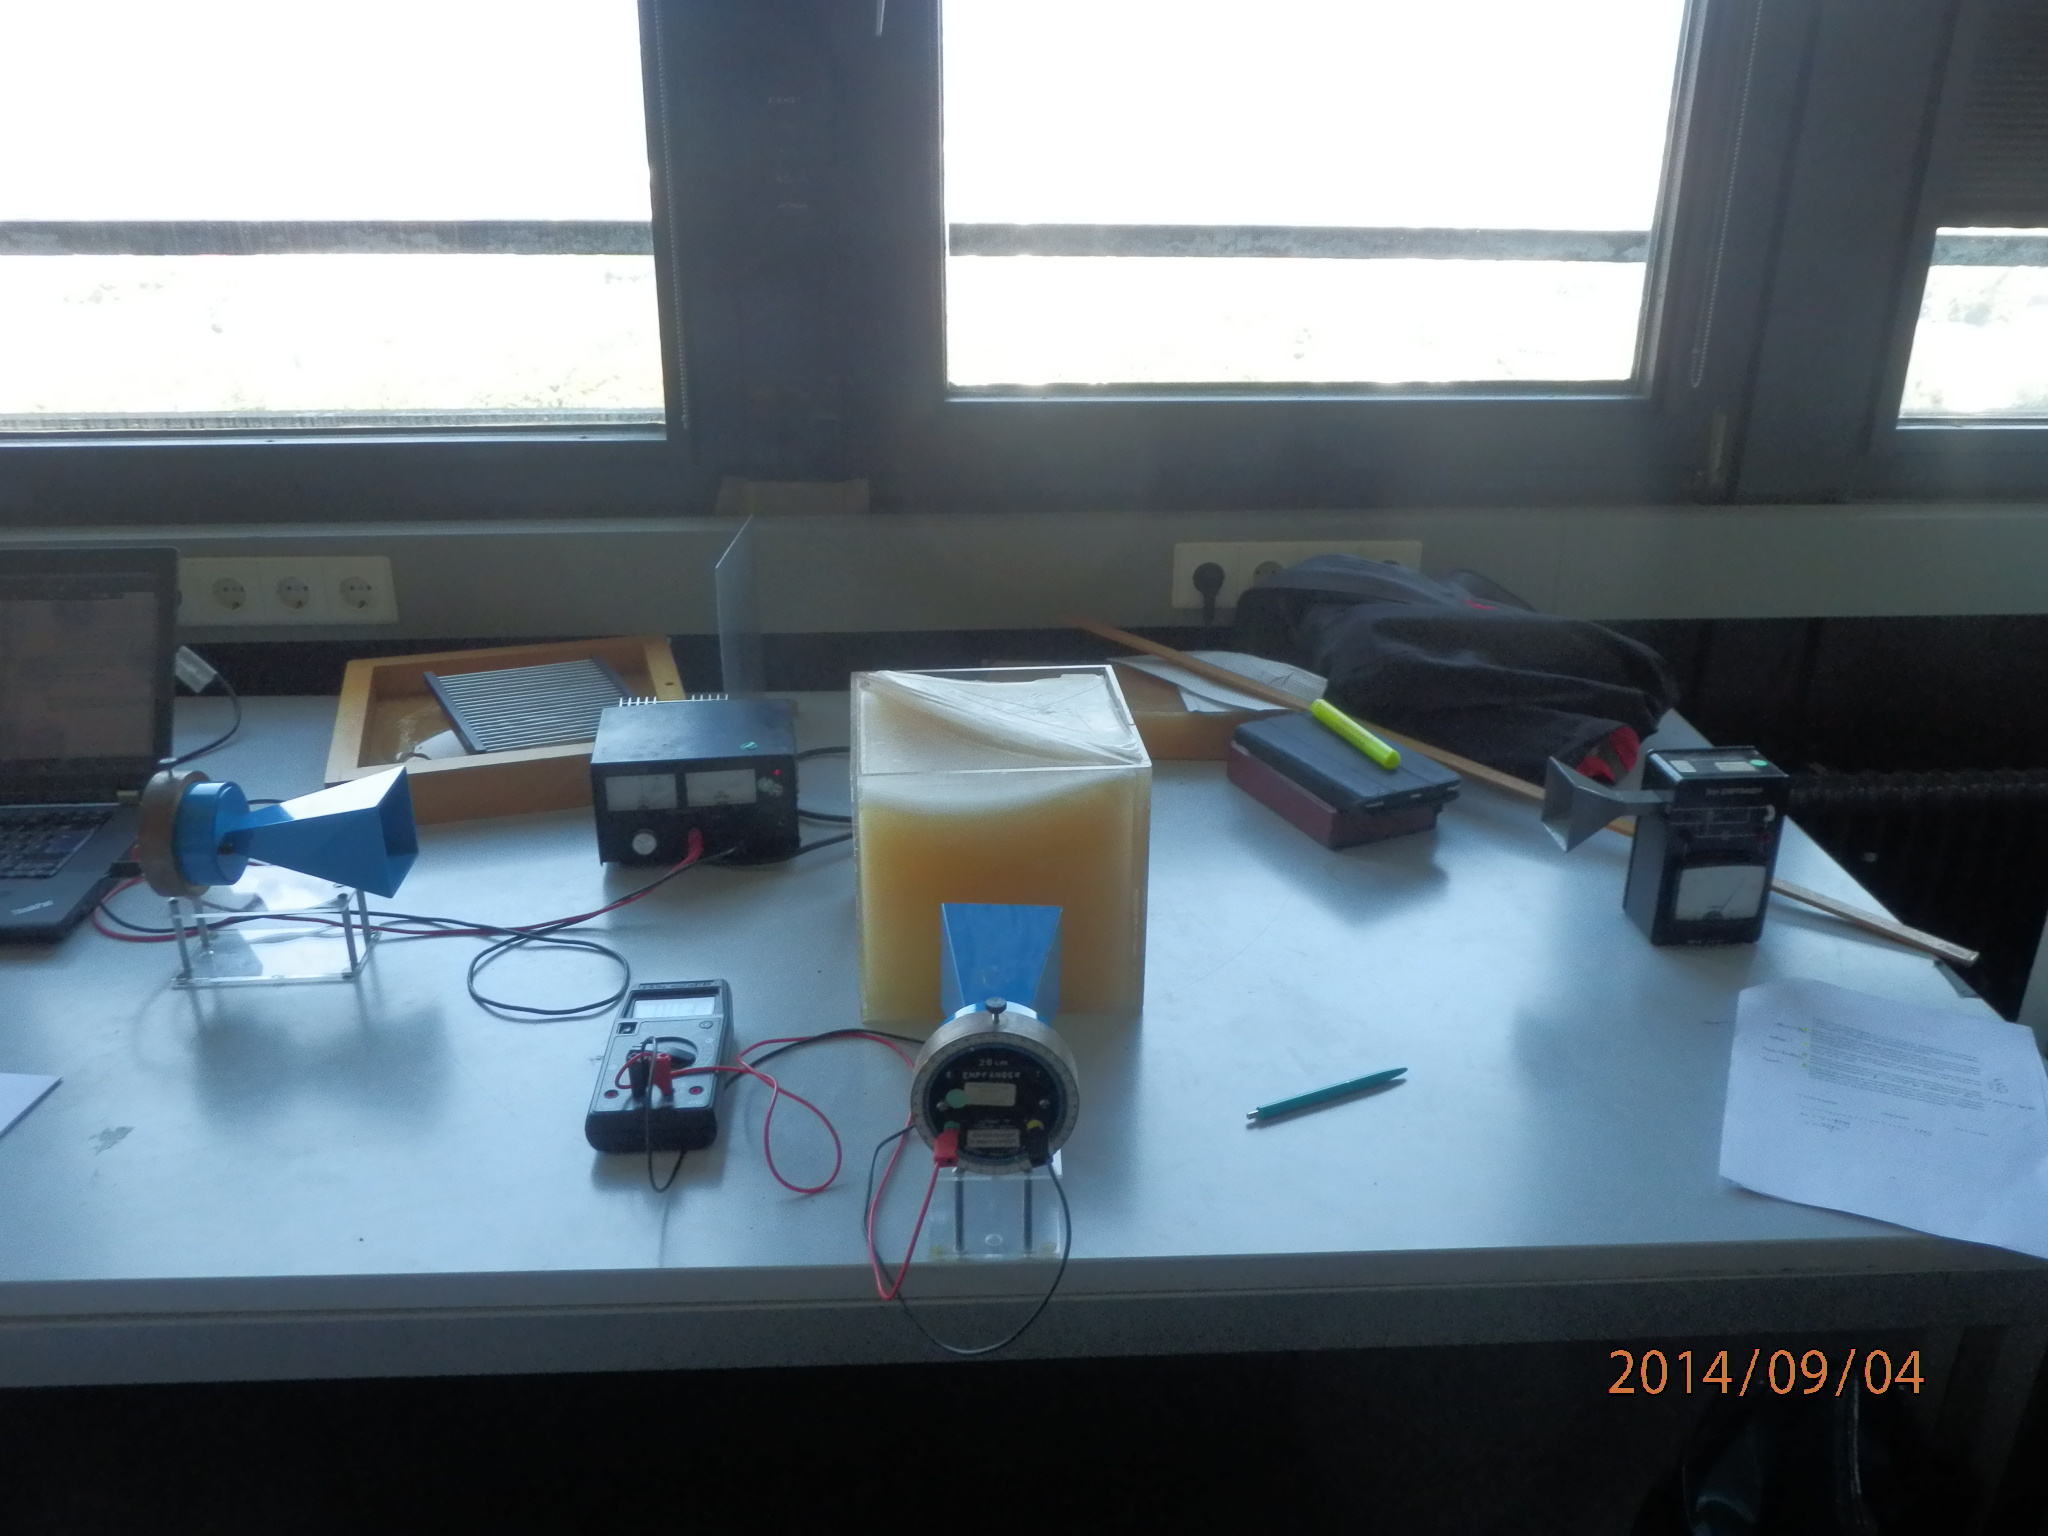
\includegraphics[scale = 0.1]{a_3.JPG}
  	\caption[Aufbau des dritten Versuchs]{Aufbau des dritten Versuchs}
  \label{fig:a_3}
\end{figure}
\subsubsection{Praktische Durchführung}
Die Totalreflexion der Mikrowellen soll anhand des folgenden Versuchs untersucht werden:

%hier die Abbildung aus der Versuchsanleitung einfügen, footnote muss noch geschrieben werden.
\begin{figure}[H] 
  \centering
    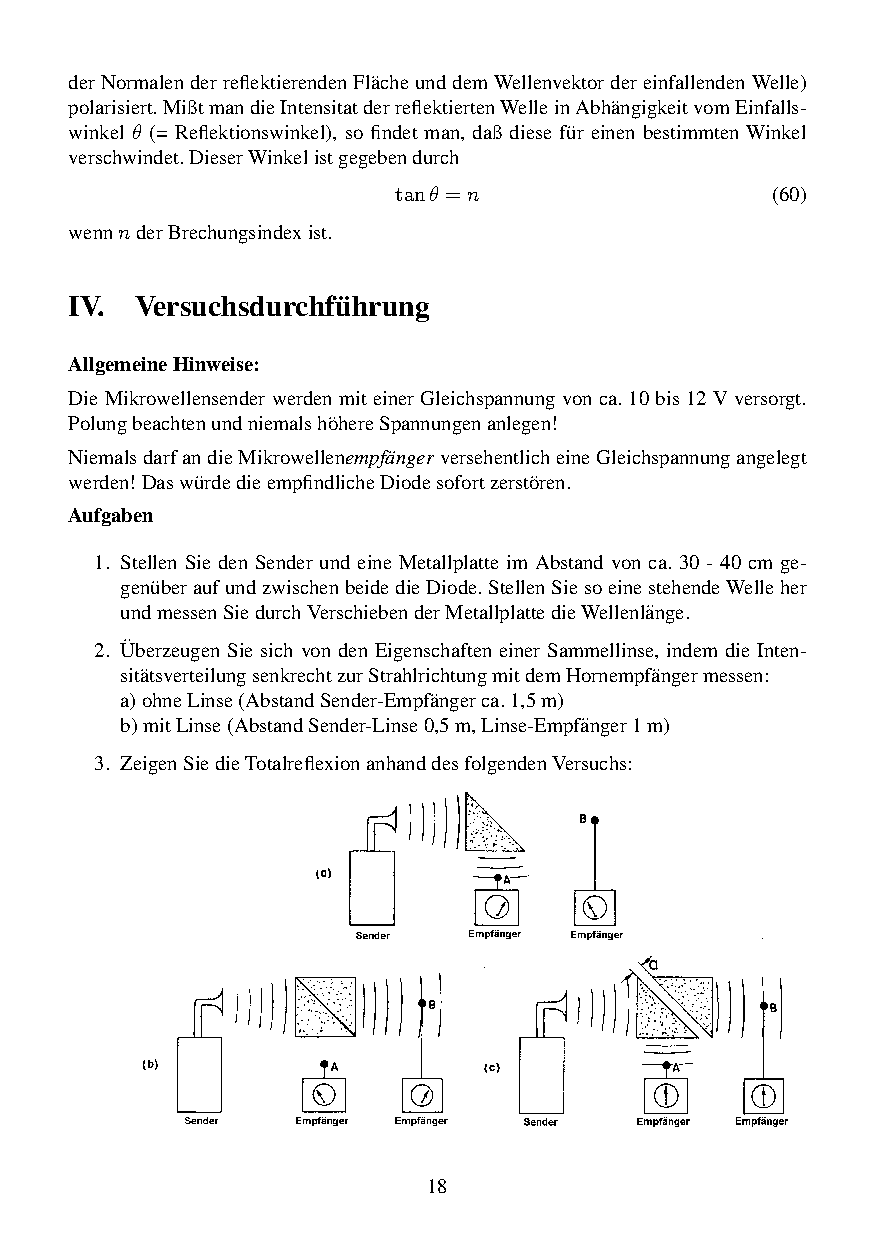
\includegraphics[trim = 0mm 15mm 0mm 132mm, clip, scale = 1]{totalreflexion.pdf}
  	\caption[Abbildung des Versuchsaufbaus zu Aufgabe 3]{Abbildung des Versuchsaufbaus zu Aufgabe 3footnotemark}
  \label{fig:abb_versuch_3}
\end{figure}
\footnotetext{Abbildung entnommen von http://www.atlas.uni-wuppertal.de/~kind/MI1.pdf Seite 18 am 03.09.2014}

Die Wachsprismen werden ( n = 1,5 ) wie in Abbildung (c) gezeichnet im Abstand a gegenüber gestellt. Wir messen nun die Intensität des Empfängers in Abhängigkeit des Abstandes a.
%Versuchen Sie, die Erscheinung zu erklären.
\subsubsection{Theoretische Durchführung}
Aufgrund der zufälligen Streuung der Welle an der Grenzschicht ist bei Empfänger A eine exponentielle Abnahme der Intensität des Lichtes mit der Vergrößerung des Abstandes der Prismen zu erwarten. Da die restliche Intensität im idealen Fall bei Empfänger B ankommt, erwarten wir erwarten wir hier eine vergleichbare Funktion mit negativem Vorzeichen und einem Versatz um eine Konstante C, welche der Anfangsintensität bei einem Abstand der Prismen von 0 cm entspricht.
\subsection{Messergebnisse}
\begin{table}[htbp]
\caption{Daten der Messung mit nur einem Block.}
\centering
\begin{tabular}{|l|l|}
\hline
Strom\_a/ $\mu$A & Strom\_b / $\mu$A \\ \hline
4 $(\pm1)$ & 140 $(\pm 5)$ \\ \hline
\end{tabular}
\label{tab:a_3_e}
\end{table}

\begin{table}[H]
\caption{Daten der Messung mit beiden Blöcken zusammen, der Fehler ist bei beiden Werten $(\pm 1)$ $\mu$A}
\centering
\begin{tabular}{|l|l|}
\hline
Strom\_a/$\mu$A & Strom\_b/$\mu$A \\ \hline
\multicolumn{1}{|r|}{81} & \multicolumn{1}{r|}{0,4} \\ \hline
\end{tabular}
\label{tab:a_3_z}
\end{table}

\begin{table}[htbp]
\caption{Daten der Messung für das auseinanderschieben der Blöcke. Der Fehler für a ist $(\pm 0,1)$ cm und für den Strom\_a $(\pm 1)$ A.}
\centering
\begin{tabular}{|r|r|r|r|}
\hline
\multicolumn{1}{|l|}{a/cm} & \multicolumn{1}{l|}{Strom\_a/$\mu$A} & \multicolumn{1}{l|}{Strom\_b/$\mu$A} \\ \hline
0,5 & 49 & 65 $(\pm 1)$ \\ \hline
1 & 29 & 90 $(\pm 2)$ \\ \hline
1,5 & 22 & 129 $(\pm 2)$ \\ \hline
2 & 19 & 147 $(\pm 4)$ \\ \hline
3 & 18 & 165 $(\pm 2)$ \\ \hline
\end{tabular}
\label{tab:a_3_m}
\end{table}
\subsection{Auswertung}
In der dritten Aufgabe sollte die Totalreflexion mit Wachsprismen bestimmt werden.
Dabei ergab sich bei der Intensitätsmessung mit nur einem Prisma  für Empfänger B ein Wert von 4 $(\pm 1) \mu$A und für Empfänger A ein Wert von 140 $(\pm 5) \mu$A.

Bei der Messung ohne Abstand zwischen den Prismen ergab sich für Empfänger B ein Wert von 0,4 $(\pm 1) \mu$A und für Empfänger A ein Wert von 81 $(\pm 1) \mu$A.

Bei der Vermessung der Intensität in Abhängigkeit des Abstandes der beiden Platten ergab sich für Empfänger A der folgende Plot (Messwerte aus Tabelle \ref{tab:a_3_m}).

\begin{figure}[H]
\centering
    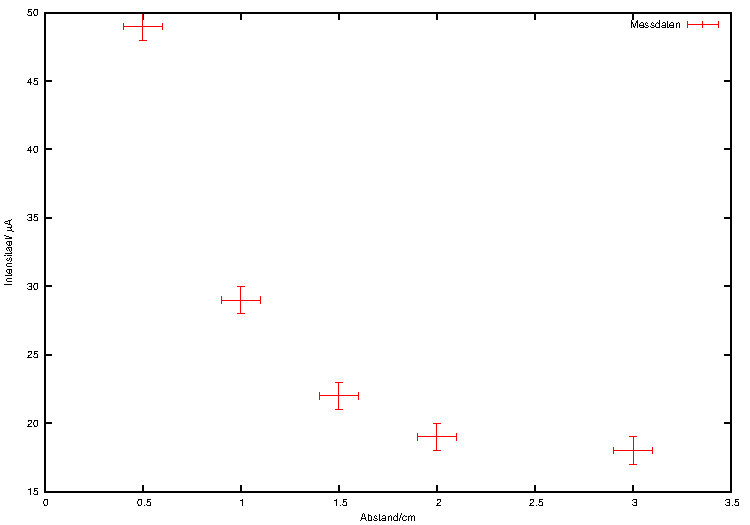
\includegraphics[scale = 1]{a_3_A.pdf}
  	\caption[Plot der Intensität an Empfänger A, in Abhängigkeit vom Abstand]{Plot der Intensität an Empfänger A, in Abhängigkeit vom Abstand}
  \label{fig:a_3_A}
\end{figure}
$f(x)= a*\exp(b*x) +c
a=-86,3 \pm 1,8; b=-2,03 \pm 0,04; c=17,72 \pm 0,18$
Für Empfänger B ergab sich der folgende Plot (Messwerte aus Tabelle \ref{tab:a_3_m} ).
Dies ergibt ein reduziertes Chiquadrat von 0,042.
\begin{figure}[H]
\centering
    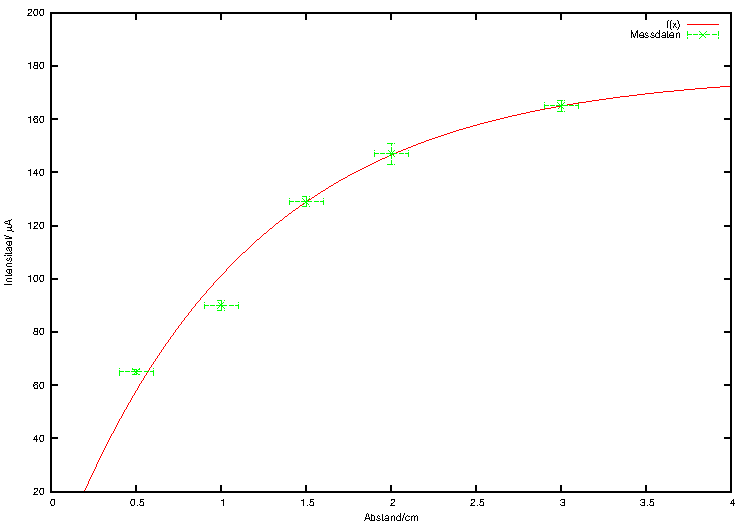
\includegraphics[scale = 1]{a_3_B.pdf}
  	\caption[Plot der Intensität an Empfänger B, in Abhängigkeit vom Abstand]{Plot der Intensität an Empfänger B, in Abhängigkeit vom Abstand}
  \label{fig:a_3_B}
\end{figure}
Hier musste manuell eine Exponentialfunktion gefittet werden, da Gnuplot beim Fitten der Funktion an die Messwerte nur Blödsinn ausspuckt:
$f(x)= a*\exp(b*(x-c)) +d
a=-100; b=-0.9; c=0.7; d=176$
Dies ergibt ein reduziertes Chiquadrat von ca.
2.25 (es wurde mit gerundeten Werten gerechnet)
%Der Fit ist mit einem reduzierten Chiquadrat von ca. 2,25  trotz der 4 freien Parameter nicht besonders gut geworden, was an einer falschen theoretischen Annahme, zu klein gewählten Fehlern oder systematische Fehlern bei der Messung liegen kann.

Dieser Effekt erklärt sich durch Streuung an der Grenzschicht begünstigt durch in Schwingung versetzte Atome und zusätzlich durch Materialinhomogenitäten.
\subsection{Diskussion}
In diesem Aufgabenteil haben wir die Totalreflektion an einem bzw. zwei Wachsprismen  gemessen. Dabei konnte man gut feststellen, dass bei kleinem Abstand der Prismen zueinander ein Teil der Welle nicht reflektiert wurde. An unsere Messdaten haben wir versucht jeweils eine Exponentialfunktion anzufitten, was im ersten Plot besser funktionierte als im zweiten. Dies resultiert aus der Vermutung, dass die Intensität des "tunnelnden" Lichtes exponentiell mit dem Abstand der Prismen abnimmt. Damit würde der restliche Teil des Lichtes bei idealen Materialeigenschaften vollständig reflektiert, was den ebenfalls exponentiellen Fit in unserem zweiten Plot erklärt. Es gab wieder Probleme mit unserem DMM, das bei Positionsänderung stark schwankende Ströme anzeigte und auch während der Messung schwankte. Dies ist durch Einflüsse des Senders der Nachbargruppe zu erklären.

\section{Aufgabe4}
\subsection{Versuchsdurchführung}
\subsubsection{Praktische Durchführung}
In dieser Aufgabe stellen wir Sender und Empfänger  so gegenüber, dass die Polarisationsrichtungen (Richtungen, in denen der E-Vektor schwingt) der beiden parallel sind. Im Folgenden drehen wir den Empfänger um die Verbindungslinie von Sender und Empfänger und messen die Intensität in Abhängigkeit des Drehwinkels.
\subsubsection{Theoretische Durchführung}
Zwischen Strom und dem Winkel, um den der Empfanger verdreht ist ist folgender Zusammenhang zu erwarten:
\begin{align}
I_s \propto \cos(\phi)
\label{eqn: Aufgabe4_cos(phi)}
\end{align}
wobei $I_s$ der gemessene Strom ist.
Zwischen Strom und Intensität gilt dabei der Zusammenhang:
\begin{align}
I_s^2 \propto I_l
\end{align}
Dabei ist $I_s$ die gemessene Stromstärke und $I_l$ die Intensität des Lichtes.
\subsection{Messergebnisse}
\begin{table}[H]
\caption{Daten der Messung für das auseinander Schieben der Blöcke. Der Fehler für a wurde mit $(\pm 0,1)$ cm und für Strom\_a mit $(\pm 1)$ A angenommen.}
\centering
\begin{tabular}{|r|r|}
\hline
\multicolumn{1}{|l|}{Winkel/grad} & \multicolumn{1}{l|}{Strom/$\mu$A} \\ \hline
0 & 191 \\ \hline
5 & 188 \\ \hline
10 & 181 \\ \hline
15 & 177 \\ \hline
20 & 174 \\ \hline
25 & 162 \\ \hline
30 & 153 \\ \hline
35 & 137 \\ \hline
40 & 119 \\ \hline
45 & 108 \\ \hline
50 & 91 \\ \hline
55 & 77 \\ \hline
60 & 63 \\ \hline
65 & 47 \\ \hline
70 & 32 \\ \hline
75 & 19 \\ \hline
80 & 9 \\ \hline
85 & 3 \\ \hline
90 & 2 \\ \hline
\end{tabular}
\label{tab:a_4}
\end{table}
\subsection{Auswertung}
In der vierten Aufgabe sollte die Intensität in Abhängigkeit des Winkels zwischen Sender und Empfänger bestimmt werden. Dabei ergab sich der folgende Plot (Messwerte aus Tabelle \ref{tab:a_4}).

\begin{figure}[H]
\centering
    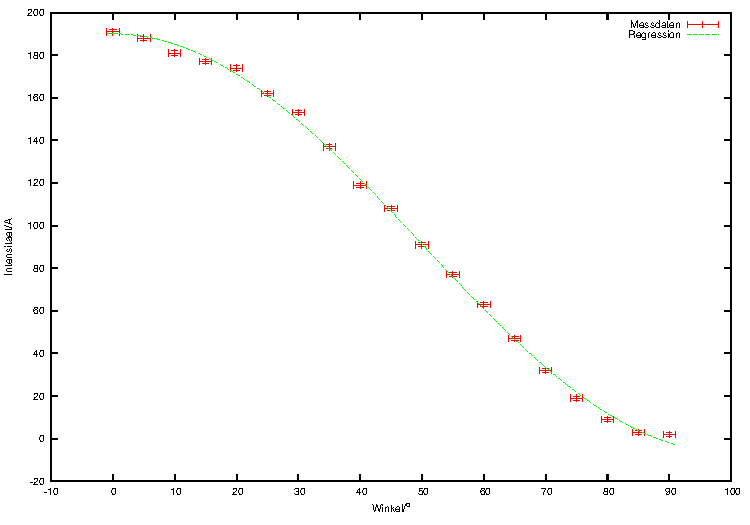
\includegraphics[scale = 1]{a_4.pdf}
  	\caption[Plot der Intensität in Abhängigkeit des Winkels zwischen Sender und Empfänger]{Plot der Intensität in Abhängigkeit des Winkels zwischen Sender und Empfänger}
  \label{fig:a_4}
\end{figure}

Die Messdaten wurden mit der der Funktion $ f(x) = m \cdot cos(x \cdot n) + b$ gefittet. Dabei ergaben sich für die Fitparameter die folgenden Werte, m = 98 $(\pm 1)$, n = 0,0315 $(\pm 0,0005)$ und b = 92 $(\pm 2)$. Das reduzierte Chiquadrat hat einen Wert von 1,52196.
\subsection{Diskussion}
In dieser Aufgabe konnte der erwartete Zusammenhang nach Formel \ref{eqn: Aufgabe4_cos(phi)} relativ gut mit den gemessenen Werten widergegeben werden.
Dies kann man gut an Abbildung \ref{fig:a_4} erkennen, wobei sich ein reduziertes Chiquadrat von ca. 1,5 ergab.
\section{Aufgabe5}
\subsection{Versuchsdurchführung}
\subsubsection{Praktische Durchführung}
Sender und Empfänger werden nun um 90$^{\circ}$ gedreht gegenüber gestellt. Ein Gitter wird so zwischen Sender und Empfänger gehalten, dass die Stäbe mit dem E-Vektor einen Winkel von 45$^{\circ}$ bilden. Wir messen bei diesem Versuchsaufbau die Intensität mit und ohne Gitter.
\subsubsection{Theoretische Durchführung}
Da der Lichtstrahl einmal durch den Polarisationsfilter und einmal durch den Empfänger abgeschwächt wird, ist der Zusammenhang
\begin{align}
I_s \propto \cos^2(\phi)
\label{eqn: Polarisationsgitter}
\end{align}
zu erwarten. (Der E-Feld-Vektor wird durch den Filter, sowie durch den Empfänger um $\cos(\phi)$ abgeschwächt. Der Winkel $\phi$ ist dabei immer der Winkel relativ zur momentanen Polarisationsrichtung des Lichtes, der in diesem Aufbau zweimal der selbe ist!)
\subsection{Messergebnisse}
\begin{table}[H]
\caption{Messdaten ohne Gitter.}
\centering
\begin{tabular}{|l|l|}
\hline
Strom/$\mu$A & Fehler/$\mu$A \\ \hline
\multicolumn{1}{|r|}{1} & \multicolumn{1}{r|}{1} \\ \hline
\end{tabular}
\label{tab:a_5_o}
\end{table}

\begin{table}[H]
\caption{Messdaten mit Gitter.}
\centering
\begin{tabular}{|l|l|}
\hline
Strom/A & Fehler/A \\ \hline
\multicolumn{1}{|r|}{86} & \multicolumn{1}{r|}{1} \\ \hline
\end{tabular}
\label{tab:a_5_m}
\end{table}
\subsection{Auswertung}
In der fünften Aufgabe sollte zwischen die um 90 Grad gegeneinander verdrehten Sender und Empfänger ein Gitter im 45 Grad Winkel zur Polarisationsrichtung gesetzt werden. Dabei ergab sich ein Wert von 1 $(\pm 1) \mu$A ohne Gitter und ein Wert von 86 $(\pm 1) \mu$A mit Gitter. Ohne verdrehen des Senders und ohne Gitter ist aus Aufgabe 4 der Wert 191 $\pm$ 2 A zu entnehmen. Wie erwartet (nach Formel \ref{eqn: Polarisationsgitter} $\phi$ = 45$^{\circ}$) hat der Strom im Vergleich zum Strom ohne Verdrehung des Senders und ohne Gitter auf ungefähr die Hälfte abgenommen (45\%).
\subsection{Diskussion}
Für einen idealen Polarisationsfilter wäre bei dieser Aufgabe nach dem Gesetz von Malus genau 50\% des Stromes nach beiden Filtervorgängen über. Die Abweichung unseres Messwertes von ca. 5\% erklärt sich einerseits durch die nicht idealen Filter, sowie andererseits durch unsere Empfangsdiode, die bei zu kleinen Amplituden Gleichströme proportional zu $E^2$ erzeugt. Es war zusätzlich ein leichter Offset von einem $\mu$A messbar. Äußere Einflüsse durch Metallische Gegenstände oder elektrische Geräte spielen hier eine recht große Rolle und verfälschen unser Ergebnis.
\section{Aufgabe6}
\subsection{Versuchsdurchführung}
\begin{figure}[H] 
  \centering
    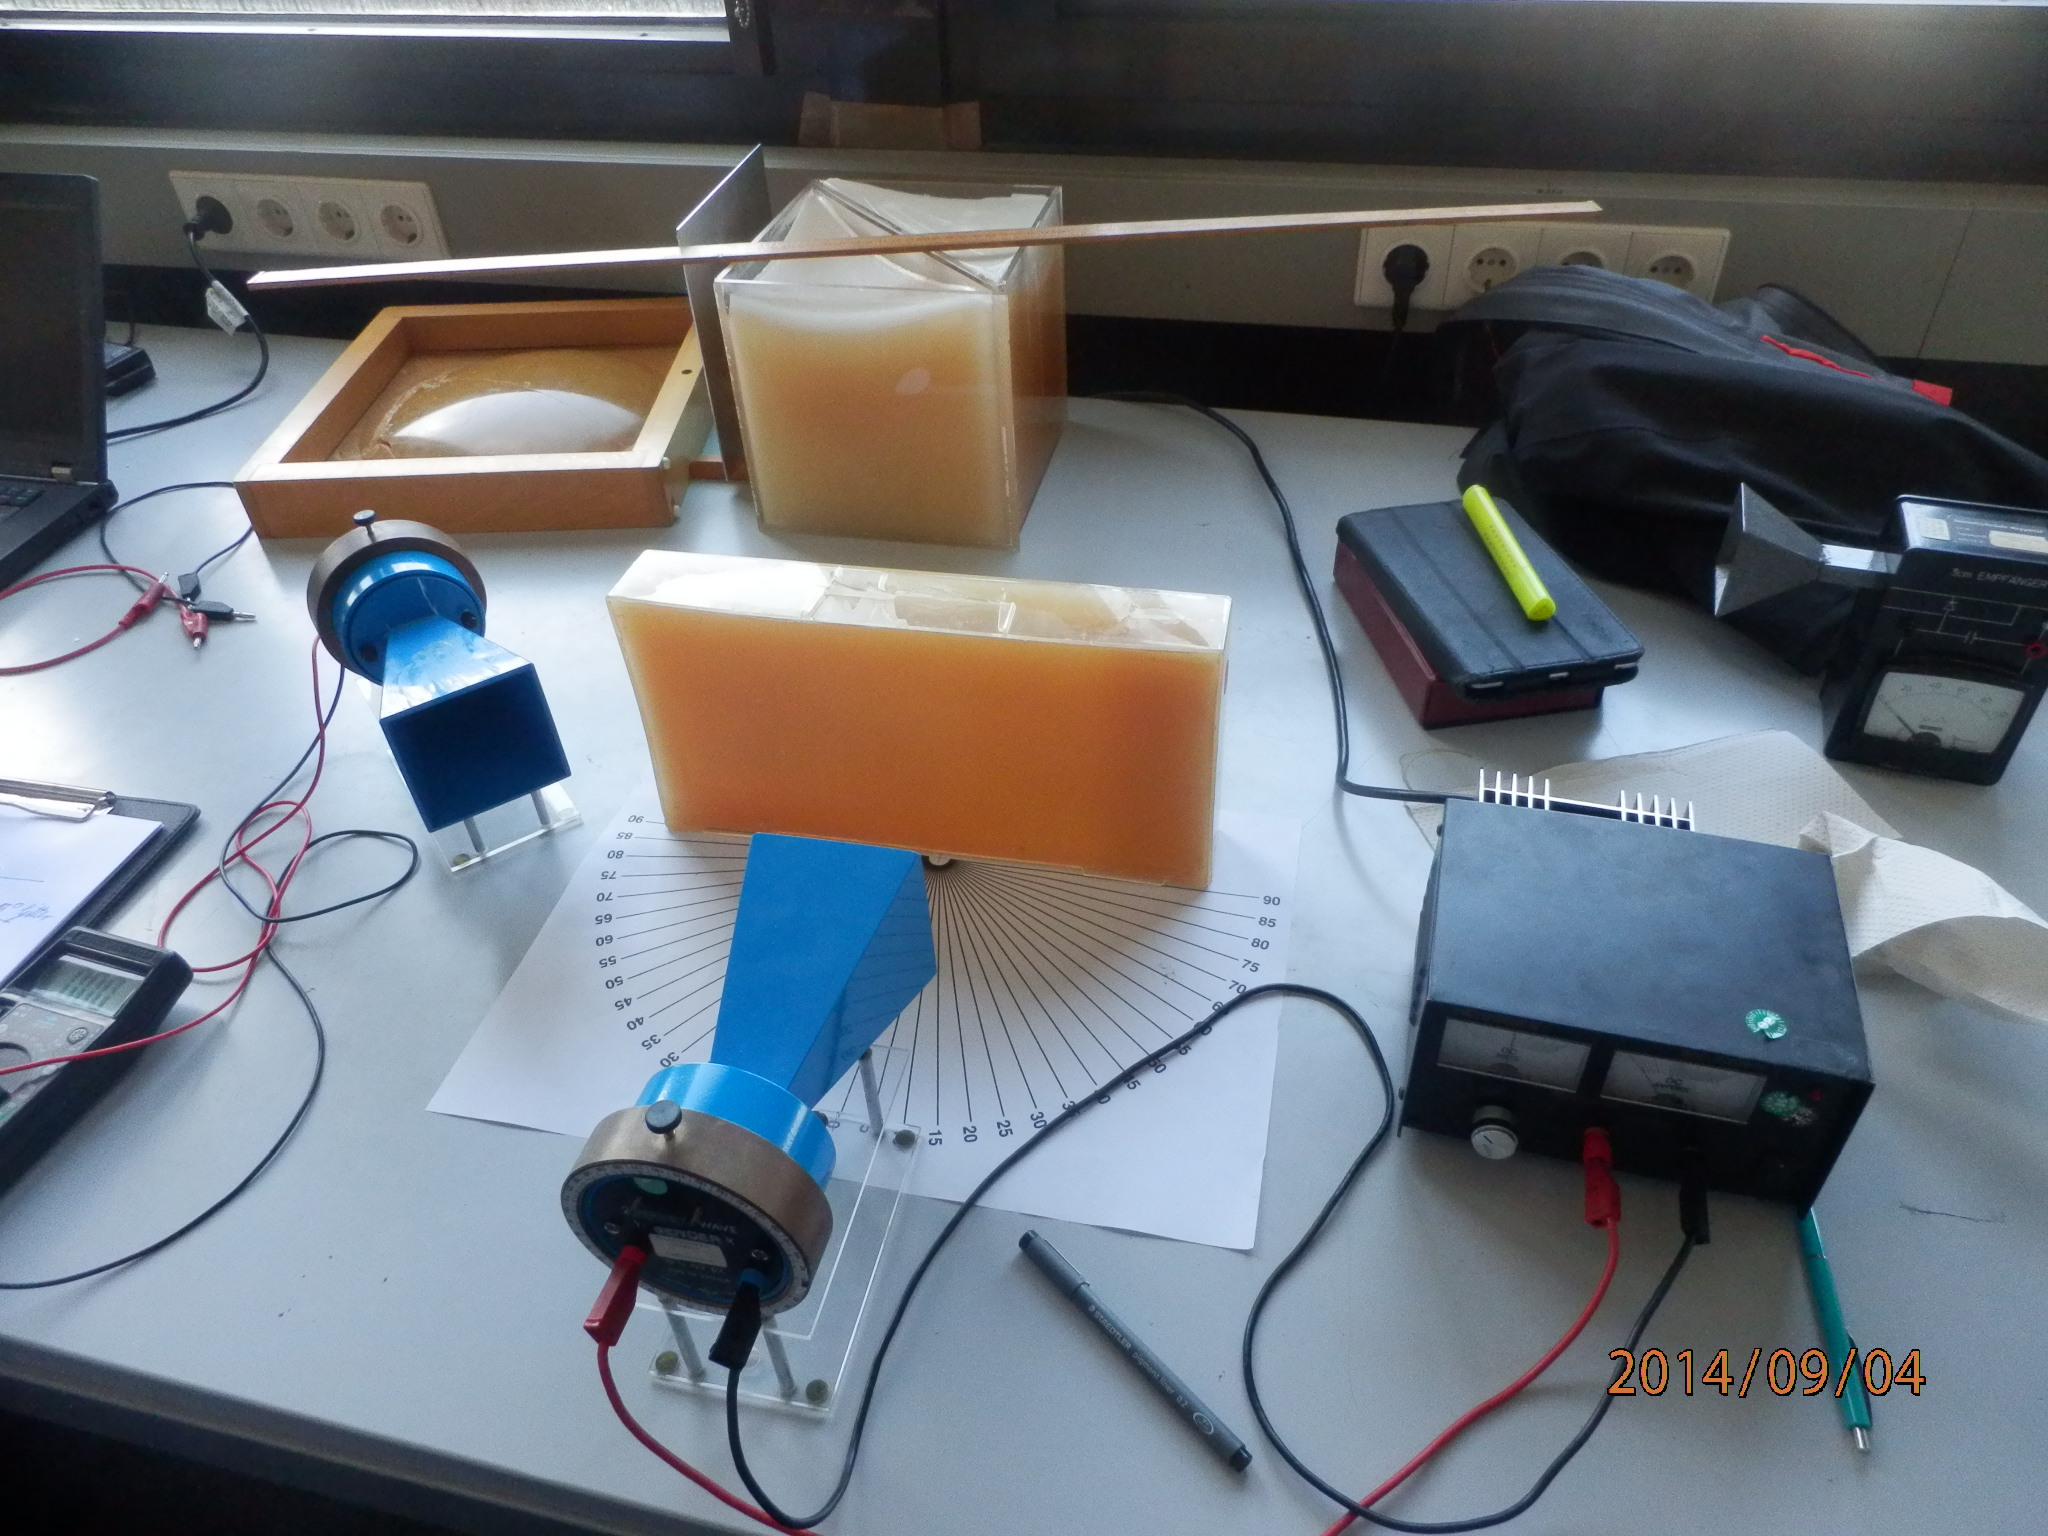
\includegraphics[scale = 0.1]{a_6.JPG}
  	\caption[Aufbau des sechsten Versuchs]{Aufbau des sechsten Versuchs}
  \label{fig:a_3}
\end{figure}
\subsubsection{Praktische Durchführung}
Abhängig vom Einfallswinkel messen wir die Intensität der von einer Wachsplatte reflektierten Wellen, die parallel zur Einfallsebene polarisiert sind. Daraus bestimmen wir den Brechungsindex.
\subsubsection{Theoretische Durchführung}
Für den Brewsterwinkel gilt die Beziehung:
\begin{align}
\tan(\phi) = \frac{n_2}{n_1}
\label{eqn: Brewsterwinkel}
\end{align}
Wobei $n_1 \cong 1$ der Brechungsindex von Luft ist. Daher wird zur Berechnung des Brechungsindex von Wachs der Nenner auf 1 gesetzt.
\subsection{Messergebnisse}
\begin{table}[H]
\caption{Messdaten für die Bestimmung des Brewsterwinkels. Der Fehler für den Winkel wurde mit $(\pm 2)^{\circ}$ und der Strom mit $(\pm 0,05)$ A angenommen.}
\centering
\begin{tabular}{|r|r|}
\hline
\multicolumn{1}{|l|}{Winkel/Grad} & \multicolumn{1}{l|}{Strom/$\mu$A} \\ \hline
10 & 0,23 \\ \hline
15 & 0,65 \\ \hline
20 & 0,45 \\ \hline
25 & 0,35 \\ \hline
30 & 1,5 \\ \hline
35 & 4 \\ \hline
40 & 6 \\ \hline
45 & 6,5 \\ \hline
50 & 8,3 \\ \hline
55 & 10,2 \\ \hline
60 & 8,8 \\ \hline
65 & 6 \\ \hline
70 & 1,85 \\ \hline
75 & 3,8 \\ \hline
80 & 8,2 \\ \hline
\end{tabular}
\label{tab:a_6}
\end{table}
\subsection{Auswertung}
In der sechsten Aufgabe sollte der Brechungsindex eines Wachsblocks über den Brewsterwinkel bestimmt werden. Dafür wurde die Intensität in Abhängigkeit vom Winkel gemessen und nach dem Winkel gesucht, für den die Intensität minimal ist. Graphisch ergab sich folgender Plot (Messwerte aus Tabelle \ref{tab:a_6}).

\begin{figure}[H]
\centering
    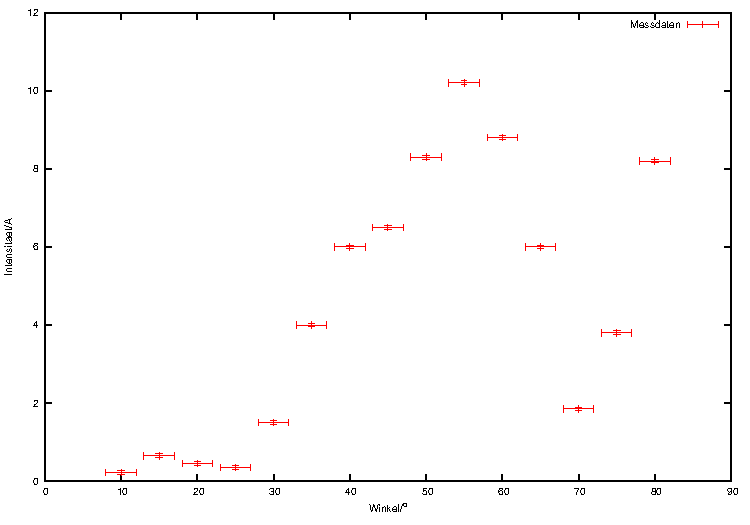
\includegraphics[scale = 1]{a_6.pdf}
  	\caption[Plot der Intensität in Abhängigkeit des Winkels]{Plot der Intensität in Abhängigkeit des Winkels}
  \label{fig:a_6}
\end{figure}
Damit kommen zwei mögliche Brewsterwinkel bei ca. 25 und 70 Grad infrage.
Nach Formel \ref{eqn: Brewsterwinkel} ergibt sich ein möglicher Brechungsindex von 0,5 $\pm$ 2,4 (25$^{\circ}$ Brewsterwinkel) sowie ein Brechungsindex von 2,7 $\pm$ 17 (70$^{\circ}$ Brewsterwinkel.) 
\subsection{Diskussion}
Da Wachs bekannterweise einen Brechungsindex von ca. 1,5 hat, was bei unserem gemessenen Maximum bei ca. 55-60 $^{\circ}$ liegt, vermuten wir, dass unsere Welle parallel zur x-y-Ebene polarisiert war, sodass wir beim Brewsterwinkel eine Maximale Reflektion gemessen haben. Die riesigen Fehler kommen daher, dass der Tangens, sowie dessen Ableitung sehr schnell gegen Unendlich geht. Dies erklärt unsere unerwarteten Messwerte und liefert im Fall der Polarisation in der x-y-Ebene einen besseren Wert für den Brewsterwinkel, welcher zudem ebenfalls einen gigantischen Fehler hat.
\section{Aufgabe7}
\subsection{Versuchsdurchführung}
\begin{figure}[H] 
  \centering
    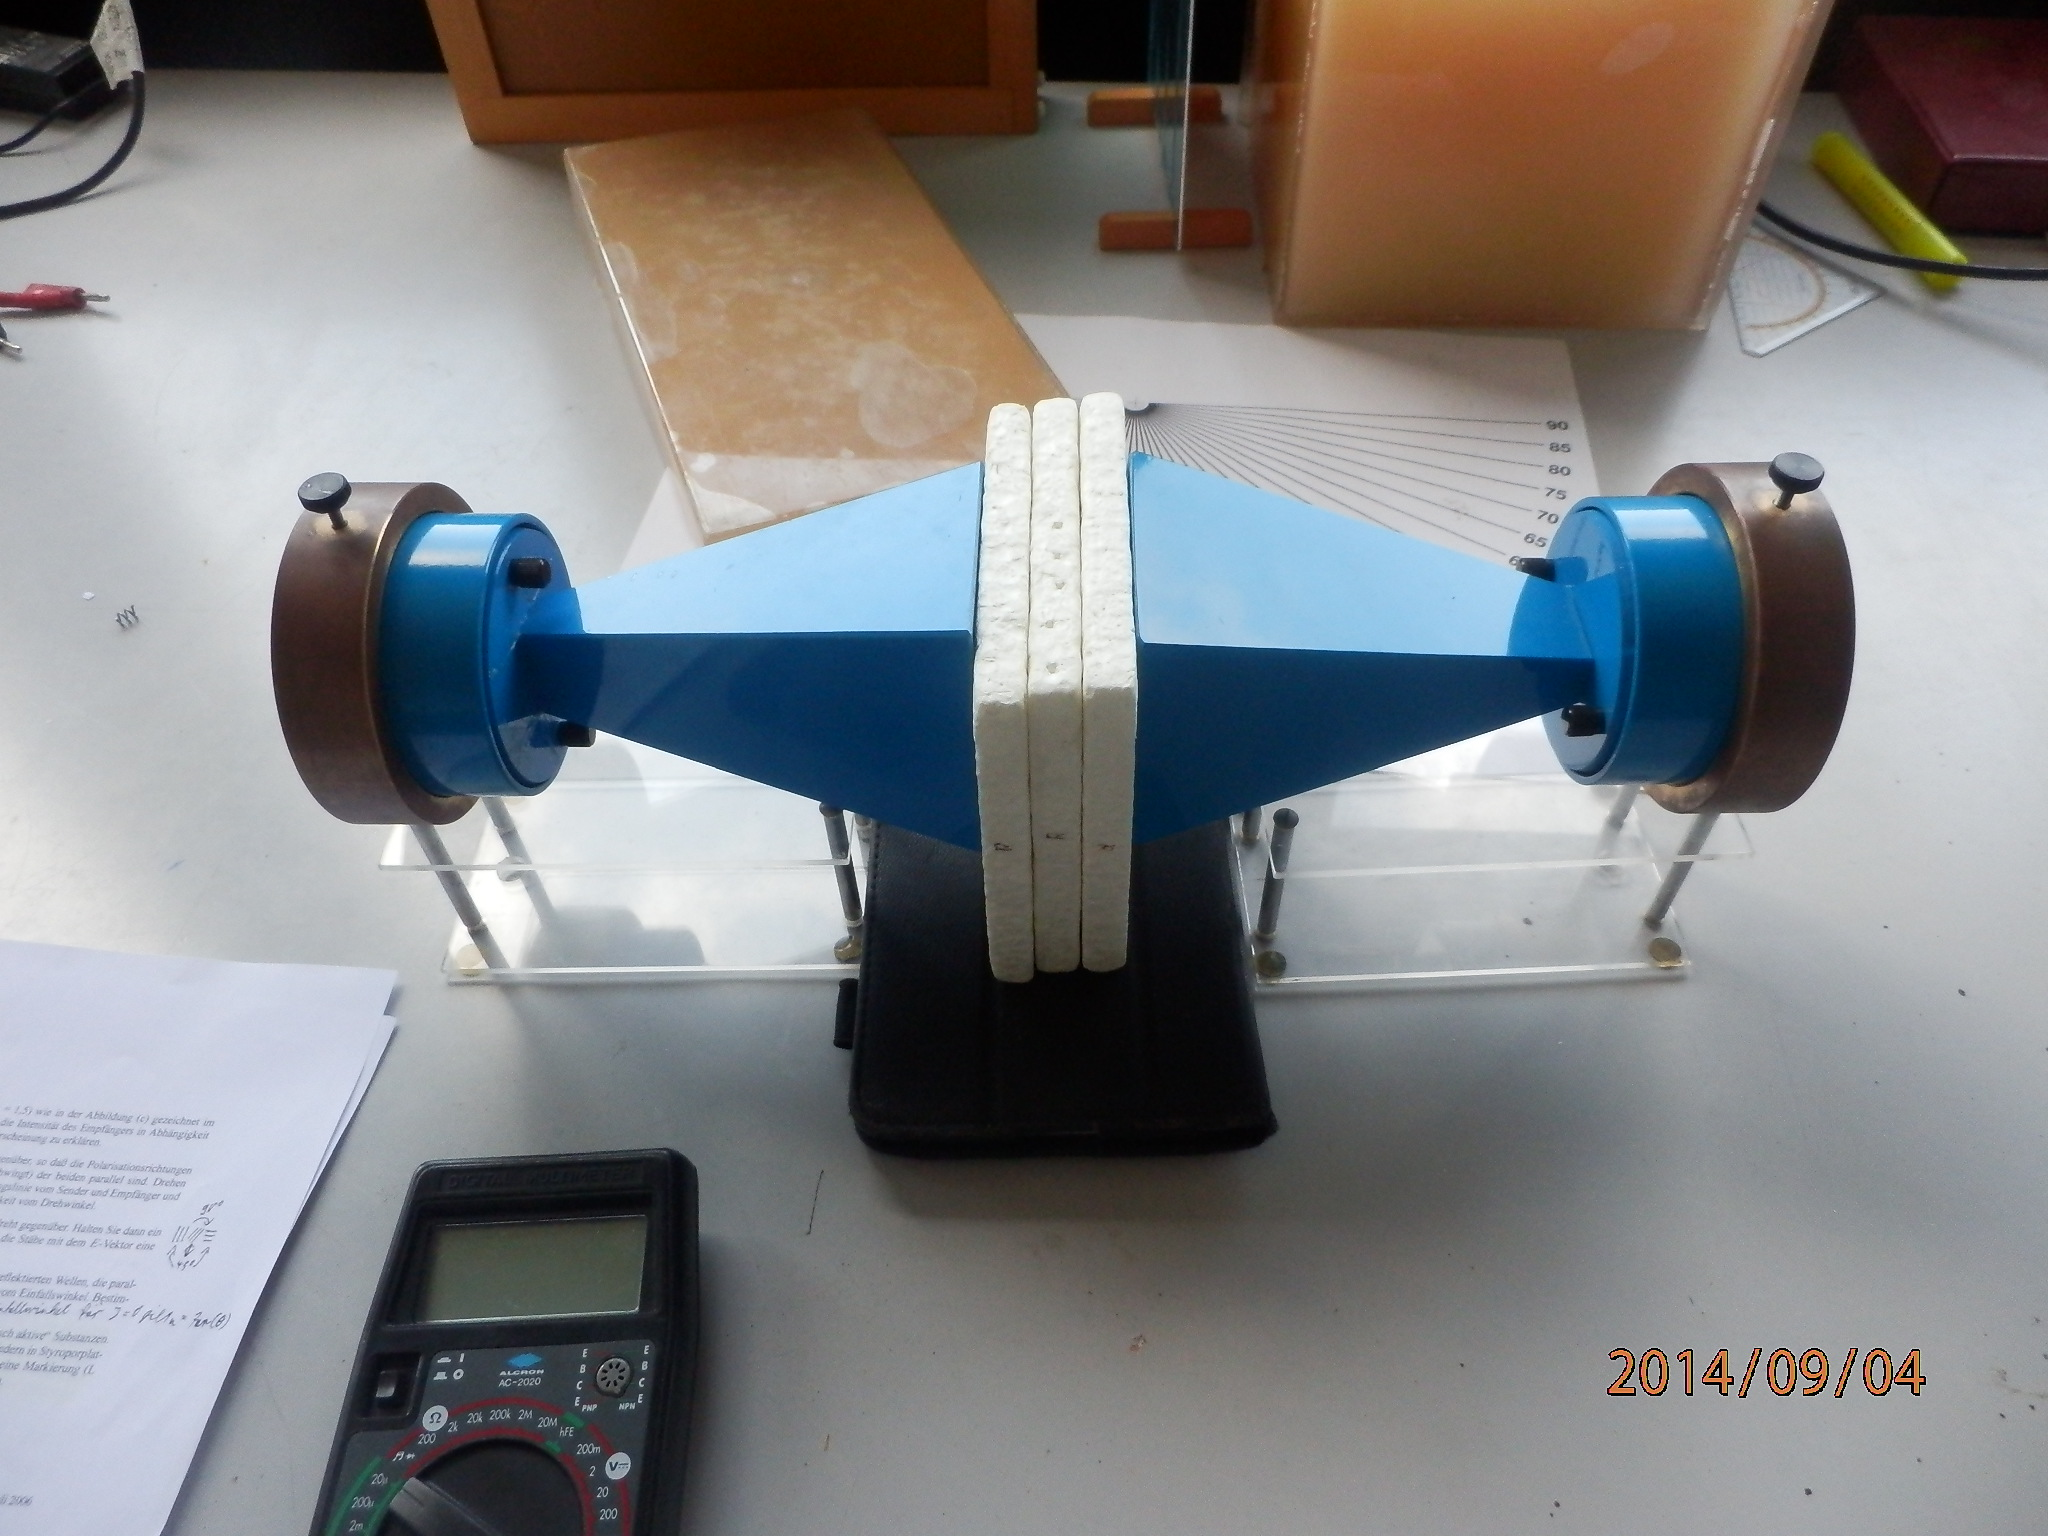
\includegraphics[scale = 0.1]{a_7.JPG}
  	\caption[Aufbau des siebten Versuchs]{Aufbau des siebten Versuchs}
  \label{fig:a_3}
\end{figure}
\subsubsection{Praktische Durchführung}
Wir wollen die Drehung der Polarisationsebene durch ”optisch aktive“ Substanzen untersuchen. Es gibt dazu optisch aktive mit Rechtsschraubenfedern besetzte Styroporplatten. Die Platten sind durch eine Markierung (R) an der Seite der Styroporplatten gekennzeichnet.
\subsection{Messergebnisse}
\begin{table}[H]
\caption{Daten der Messung ohne Styropor (mit Rechtsschraubenfedern versehen).}
\centering
\begin{tabular}{|l|l|l|l|}
\hline
Strom/$\mu$A & Fehler/$\mu$A & Winkel/grad & Fehler/grad \\ \hline
\multicolumn{1}{|r|}{0,8} & \multicolumn{1}{r|}{0,05} & \multicolumn{1}{r|}{90} & \multicolumn{1}{r|}{1} \\ \hline
\end{tabular}
\label{tab:a_7_o}
\end{table}

\begin{table}[H]
\caption{Daten der Messung mit Styropor (mit Rechtsschraubenfedern versehen).}
\centering
\begin{tabular}{|r|r|r|r|}
\hline
\multicolumn{1}{|l|}{Strom/$\mu$A} & \multicolumn{1}{c|}{Fehler/$\mu$A} & \multicolumn{1}{l|}{Winkel/Grad} & \multicolumn{1}{l|}{Fehler/Grad} \\ \hline
3,2 & 0,05 & 90 & 1 \\ \hline
0,8 & 0,005 & 97 & 1 \\ \hline
\end{tabular}
\label{tab:a_7_m}
\end{table}
\subsection{Auswertung}
In der siebten Aufgabe sollte der Effekt optisch aktiver Substanzen nachgewiesen werden. Dafür wurden Sender und Empfänger um 90 $(\pm 1)$ Grad zueinander verdreht und die Intensität gemessen. Dabei ergab sich ein Wert von 0,81 $(\pm 0,05) \mu$A.  Dann wurde die optisch aktive Substanz (Styropor mit Stahlfedern) zwischen Sender und Empfänger gehalten und der Sender solange nach links gedreht,bis sich der zuvor bestimmte Wert einstellte. Es ergab sich ein Winkel von 97 $(\pm 1)$ Grad.
\subsection{Diskussion}
Da es keine Materialangaben zum mit Stahlfedern besetzten Styropor gab, können wir unser Ergebnis nicht direkt vergleichen. Andere Gruppen haben jedoch ähnliche Werte gemessen, was dafür spricht, dass der Messwert in Ordnung ist.
\section{Fazit}
Abschließend betrachtet sind fast alle Messungen zufriedenstellend verlaufen. Lediglich bei Aufgabe 6 ist das Ergebnis stark vom erwarteten Wert abgewichen. Neben dem riesigen Fehlerterm auf unsere errechneten Brechungsindizes ist dies dadurch zu erklären, dass die Mikrowellen möglicherweise parallel zur x-y-Ebene  polarisiert waren.
Wir hatten in fast allen Versuchsteilen während den Strommessungen Probleme mit unsere DMM, welches beim umschalten auf andere Zehnerpotenzen andere Ströme anzeigte.
Neben äußeren Einflüssen wie z.b vom Sender der Nachbargruppe zeigten unsere Wachsprismen in Aufgabe 3 je nach Position der Empfanger andere Eigenschaften (der Strom variierte abhängig von der Posiiton des Empfängers stark, was sich nur mit einigen Inhomogenitäten unsers Materials erklären lässt. 
Die restlichen Messungen haben soweit alle erwarteten optischen Effekte bestätigt.

 %Werte stimmen mit den Formeln überein/nicht überein

\end{document}

